
\setlength{\columnsep}{3pt}
\begin{flushleft}
	\bigskip
	\begin{itemize}
		\item \textbf{Authoritative nameserver}:
		\begin{itemize}
			\item An authoritative nameserver has the original settings for domain name.
			\item This is where the domain administrator has configured the DNS records for a domain. 
			
			\begin{figure}[h!]
				\centering
				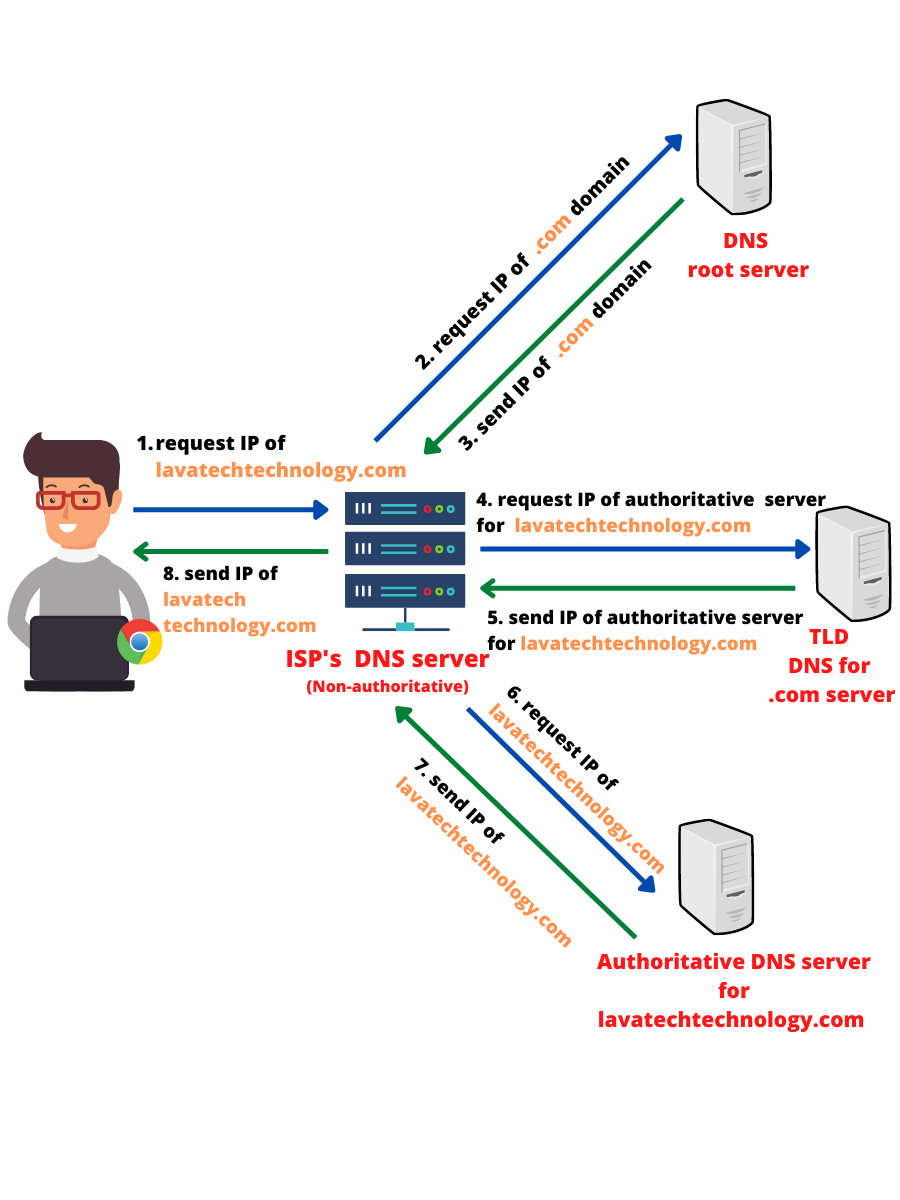
\includegraphics[scale=.48]{content/chapter3/images/auth.png}
				\caption{DNS Hierarchy}
				\label{fig:dns_heir}
			\end{figure}
			\newpage
			\item Find authoritative DNS server for any domain:
			\begin{tcolorbox}[breakable,notitle,boxrule=0pt,colback=pink,colframe=pink]
				\color{black}
				\fontdimen2\font=1em
				Syntax: dig +short NS <domain name>
				\fontdimen2\font=4pt
			\end{tcolorbox}
			Eg:
			\begin{tcolorbox}[breakable,notitle,boxrule=-0pt,colback=black,colframe=black]
				\color{green}
				\fontdimen2\font=1em
				\# dig +short NS lavatechtechnology.com
				\newline
				\color{white}
				ns06.domaincontrol.com.
				\newline
				ns05.domaincontrol.com.
				\fontdimen2\font=4pt
			\end{tcolorbox}
			
			or 
			\begin{tcolorbox}[breakable,notitle,boxrule=0pt,colback=pink,colframe=pink]
				\color{black}
				\fontdimen2\font=1em
				Syntax: host -t ns <domain name>
				\fontdimen2\font=4pt
			\end{tcolorbox}
			Eg:
			\begin{tcolorbox}[breakable,notitle,boxrule=-0pt,colback=black,colframe=black]
				\color{green}
				\fontdimen2\font=1em
				\# host -t ns lavatechtechnology.com
				\newline
				\color{white}
				lavatechtechnology.com name server ns06.domaincontrol.com.
				\newline
				lavatechtechnology.com name server ns05.domaincontrol.com.
				\fontdimen2\font=4pt
			\end{tcolorbox}
			
			\bigskip
			\item Using \textbf{nslookup} (\textbf{N}ame \textbf{S}erver lookup) command, confirm if the domain name is resolved using the authoritative nameserver.
			\begin{tcolorbox}[breakable,notitle,boxrule=0pt,colback=pink,colframe=pink]
				\color{black}
				\fontdimen2\font=1em
				Syntax: nslookup <domain-name> <nameserver>
				\fontdimen2\font=4pt
			\end{tcolorbox}
			
			\begin{figure}[h!]
				\centering
				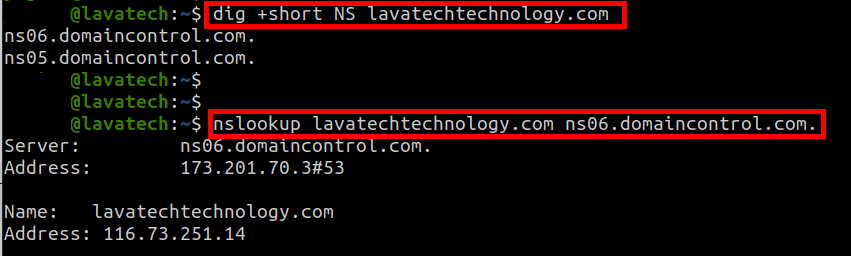
\includegraphics[scale=.35]{content/chapter3/images/ans.png}
				\caption{Sample output}
				\label{fig:dns_heir3}
			\end{figure}			
		
		\end{itemize}
		
		\newpage
		\item \textbf{Non-authoritative nameserver}:
		\begin{itemize}
			\item Non-authoritative name servers do not contain original source files of domain’s zone. 
			\item They have a \textbf{cache file} for the domains that is constructed from all the DNS lookups done previously. 
			\item If a DNS server responded for a DNS query which doesn’t have original file is known as a Non-authoritative answer.
			\item Find non-authoritative DNS server for any domain:
			\begin{tcolorbox}[breakable,notitle,boxrule=0pt,colback=pink,colframe=pink]
				\color{black}
				\fontdimen2\font=1em
				Syntax: nslookup <domain-name>
				\fontdimen2\font=4pt
			\end{tcolorbox}
			Eg:
			\begin{tcolorbox}[breakable,notitle,boxrule=-0pt,colback=black,colframe=black]
				\color{green}
				\fontdimen2\font=1em
				\# nslookup lavatechtechnology.com
				\fontdimen2\font=4pt
			\end{tcolorbox}
			
			\begin{figure}[h!]
				\centering
				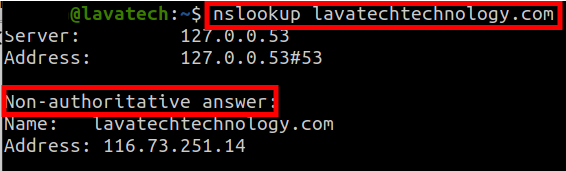
\includegraphics[scale=.5]{content/chapter3/images/ns1.png}
				\caption{Sample output}
				\label{fig:dns_heir4}
			\end{figure}			

			\begin{figure}[h!]
				\centering
				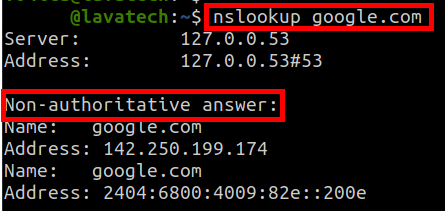
\includegraphics[scale=.6]{content/chapter3/images/ns2.png}
				\caption{Sample output}
				\label{fig:dns_heir5}
			\end{figure}			
			
		\end{itemize}
		
		
		
		\item \textbf{}:
	
	\end{itemize}
\end{flushleft}

\newpage





